
\begin{figure}[t]
	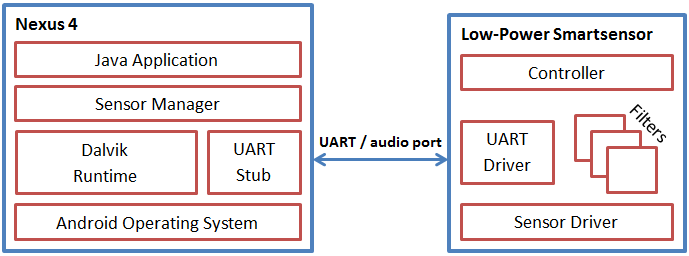
\includegraphics[width=3.1in]{prototype_architecture.png}
	\caption{Prototype architecture.}
    \label{fig:prototypeArchitecture}
\end{figure}

\section{Prototype}
\label{sec:prototype}

We implemented a prototype of our system using a Google Nexus 4 phone
running Android 4.2.2.  The low-power Smartsensor is implemented using
a Texas Instruments micro-controller board attached to an
accelerometer sensor.  We chose to focus our efforts on the
accelerometer sensor because of its relative simplicity and the
availability of a wide range of accelerometer-based applications on
various mobile application markets.  Figure
\ref{fig:prototypeArchitecture} shows a high-level diagram of the
prototype's architecture.

The Nexus 4 and TI board communicate over the UART port made available
by the Nexus 4 debugging interface via the physical port used by the
audio interface.  The serial connection provides sufficient bandwidth
to support low bit-rate sensors, such as the accelerometer, a
microphone or GPS.  However, extending the prototype to work with
higher bit-rate sensors like the camera would require a higher
bandwidth data bus, such as $I^2C$.

The rest of this section describes our extensions to the phone, the
implementation of the Smartsensor board, and the applications and test
frameworks we use in our experiments.

\subsection{Nexus 4}
\label{subsec:nexus}

\begin{figure*}[t]
{\small
	\begin{verbatim}
		SensorManager mSensorMan = (SensorManager) getSystemService(Context.SENSOR_SERVICE);
		Sensor mAccelerometer = mSensorMan.getDefaultSensor(Sensor.TYPE_ACCELEROMETER);
		mSensorMan.registerListener(new MySensorEventListener(), mAccelerometer);
	\end{verbatim}
}
	\caption{Typical usage of Android's SensorManager}
    \label{fig:androidSensorCodeNormal}
\end{figure*}

\begin{figure*}[t]
{\small
	\begin{verbatim}
		SensorManager mSensorMan = (SensorManager) getSystemService(Context.SENSOR_SERVICE);
		Sensor mAccelerometer = mSensorMan.getSmartSensor(Sensor.TYPE_ACCELEROMETER);
		DataFilterAlgorithm mDataFilter = new ExponentialMovingAverageLowPassFilter(0.75);
		WakeUpCondition mWakeUpCond = new MinThresholdWakeUpCondition(mDataFilter, Sensor.AXIS_X, 12.0);
		mSensorMan.registerListener(new MySensorEventListener(), mAccelerometer, mWakeUpCond);
	\end{verbatim}
}
	\caption{Usage of the SensorManager with a wake-up condition.}
    \label{fig:androidSensorCodeModified}
\end{figure*}

On the Nexus phone we extended Android's SensorManager to include the
new features made available by our system. To prevent a steep learning
curve, our goal was to provide an API very similar to Android's
existing sensors API.  

We extended the Sensor Manager to allow users to define custom wake-up
conditions by specifying a pre-defined data filter and configuring the
filter and wake-up parameters. The available types of sensor data filters, 
described in detail in Subsection
\ref{sec:sensorDataFilters}, are a set of predefined implementations
of a DataFilterAlgorithm interface.
Figures~\ref{fig:androidSensorCodeNormal}
and~\ref{fig:androidSensorCodeModified} show an example of an
application that registers a listener to receive accelerometer
readings using the default Android Sensor Manager, and the modified
code that includes a wake-up condition that uses an exponential moving
average low-pass filter and an x-axis threshold, respectively.

We also created a UART stub to facilitate communication between the
mobile phone and the Smartsensor board. The UART stub is called when
the Smartsensor board detects an event based on its wake-up condition.
In turn, the UART stub is a shell script that notifies the
SensorManager using an Android Intent\cite{androidintents}.

For our prototype we avoid modifying the Android kernel in any way.
Because the current prototype uses the UART port for communication
with the Smartsensor, we were able to constrain our implementation to
the user space. An integrated implementation would likely make use of
a higher bandwidth bus such as the $I^2C$ bus and require a custom
driver.


\begin{table*}[t]
{\small
	\begin{tabular}{| p{7cm} | l | l |}
		\hline
		State & Average Power Consumption (mW) & Average Duration \\ \hline
	%    TI MSP430 & Awake & 3.6 & N/A \\ \hline
	%    TI Stellaris & Awake & 49.4 & N/A \\ \hline
		Awake, running a pedometer application with data from the internal accelerometer & 323 & N/A \\ \hline
		Asleep & 9.7 & N/A \\ \hline
		Asleep-to-Awake Transition & 384 & 1 second \\ \hline
		Awake-to-Asleep Transition & 341 & 1 second \\ \hline
	\end{tabular}
}
	\caption{Google Nexus 4 power profile.}
	\label{table:powerProfileNexus}
\end{table*}

We power profiled the Google Nexus 4. The results are summarized in
Table \ref{table:powerProfileNexus}. During all the measurements, the
device's screen, WiFi and GPS were turned off.  While the device is
sleeping, its power usage is very low, consuming only 9.7 mW. While
awake, the power consumption is significantly higher, averaging 323
mW. During our power measurements we noticed that additional energy is
consumed during transitions between the asleep and awake states. Each
transition takes about 1 second. During a wake-up transition, the
average power consumption goes up to 384 mW, while during an
awake-to-asleep transition the average power consumption is 341 mW.


\subsection{Smartsensor Board}
\label{subsec:sensorBoard}

The low-power Smartsensor board consists of a driver that talks to
the accelerometer sensor, a set of filtering algorithms, a controller,
and an UART driver for communicating with the phone. The controller
orchestrates the execution of the filters, and uses the UART driver to
wake up the phone when a wake-up condition is satisfied.  The UART driver
opens a serial port and then uses a TTY to copy the sensor readings
and start the shell script that notifies the Sensor Manager.


\subsubsection{Sensor Data Filters}
\label{sec:sensorDataFilters}

We implemented three filters of increasing complexity:

\paragraph{Null} This algorithm performs no filtering.  It simply
  forwards the raw accelerometer readings.


  \paragraph{EMA} Applies an exponential moving average low-pass
  filter that removes some of the noise from the sensor data and is
  computationally cheap, requiring only a few algebraic operations for
  every sensor reading. The filter takes an alpha parameter between 0
  and 1, that controls the ``smoothness'' of the filtered data, and
  implements the following equation: $out_{t} = (1-\alpha) \times
  out_{t-1} + \alpha \times in$

  \paragraph{FFT} Applies a low-pass filter based on Fast Fourier
  transformations~\cite{libbyFootstepDetection} that is more accurate
  at removing noise from the sensor data. However, it is
  computationally expensive. Two parameters can be set for the
  FFT: a window-size and a relative energy threshold value. The
  window size indicates the number of readings that are to be used in
  each discrete Fourier transform. The relative energy threshold value
  controls the amount of energy in the output data. A lower relative
  energy threshold value would result in ``smoother'' output sensor
  values.

\subsubsection{Wake-up conditions}

Programmers specify a wake-up condition by selecting a filtering
algorithm and setting one or more thresholds.  The prototype supports
the following thresholds:

\paragraph{Minimum Threshold} is satisfied when the acceleration exceeds the threshold value

\paragraph{Maximum Threshold} is satisfied when the acceleration goes below the threshold value

\paragraph{Threshold Range} is satisfied when the acceleration is between two threshold values


\subsubsection{Hardware Options}

We evaluated two low-power micro-controllers manufactured by Texas
Instruments, the MSP430 and the Stellaris LM4F120H5QR.  The MSP430 has
the advantage of requiring very little power, consuming only 3.6 mW
while awake. However, it has limited memory and cannot perform complex
analysis of sensor data in real-time. In our tests, it was unable to
run the FFT-based low-pass filter in real-time.  The Stellaris LM4F120H5QR is powered
by a Cortex-M4 processor. It can batch a higher number of accelerometer
readings and can run all our filters in real-time.  However, this
micro-controller has an energy footprint an order of magnitude greater
than the MSP430, consuming an average of 49.4 mW while awake.

\begin{figure}[t]
	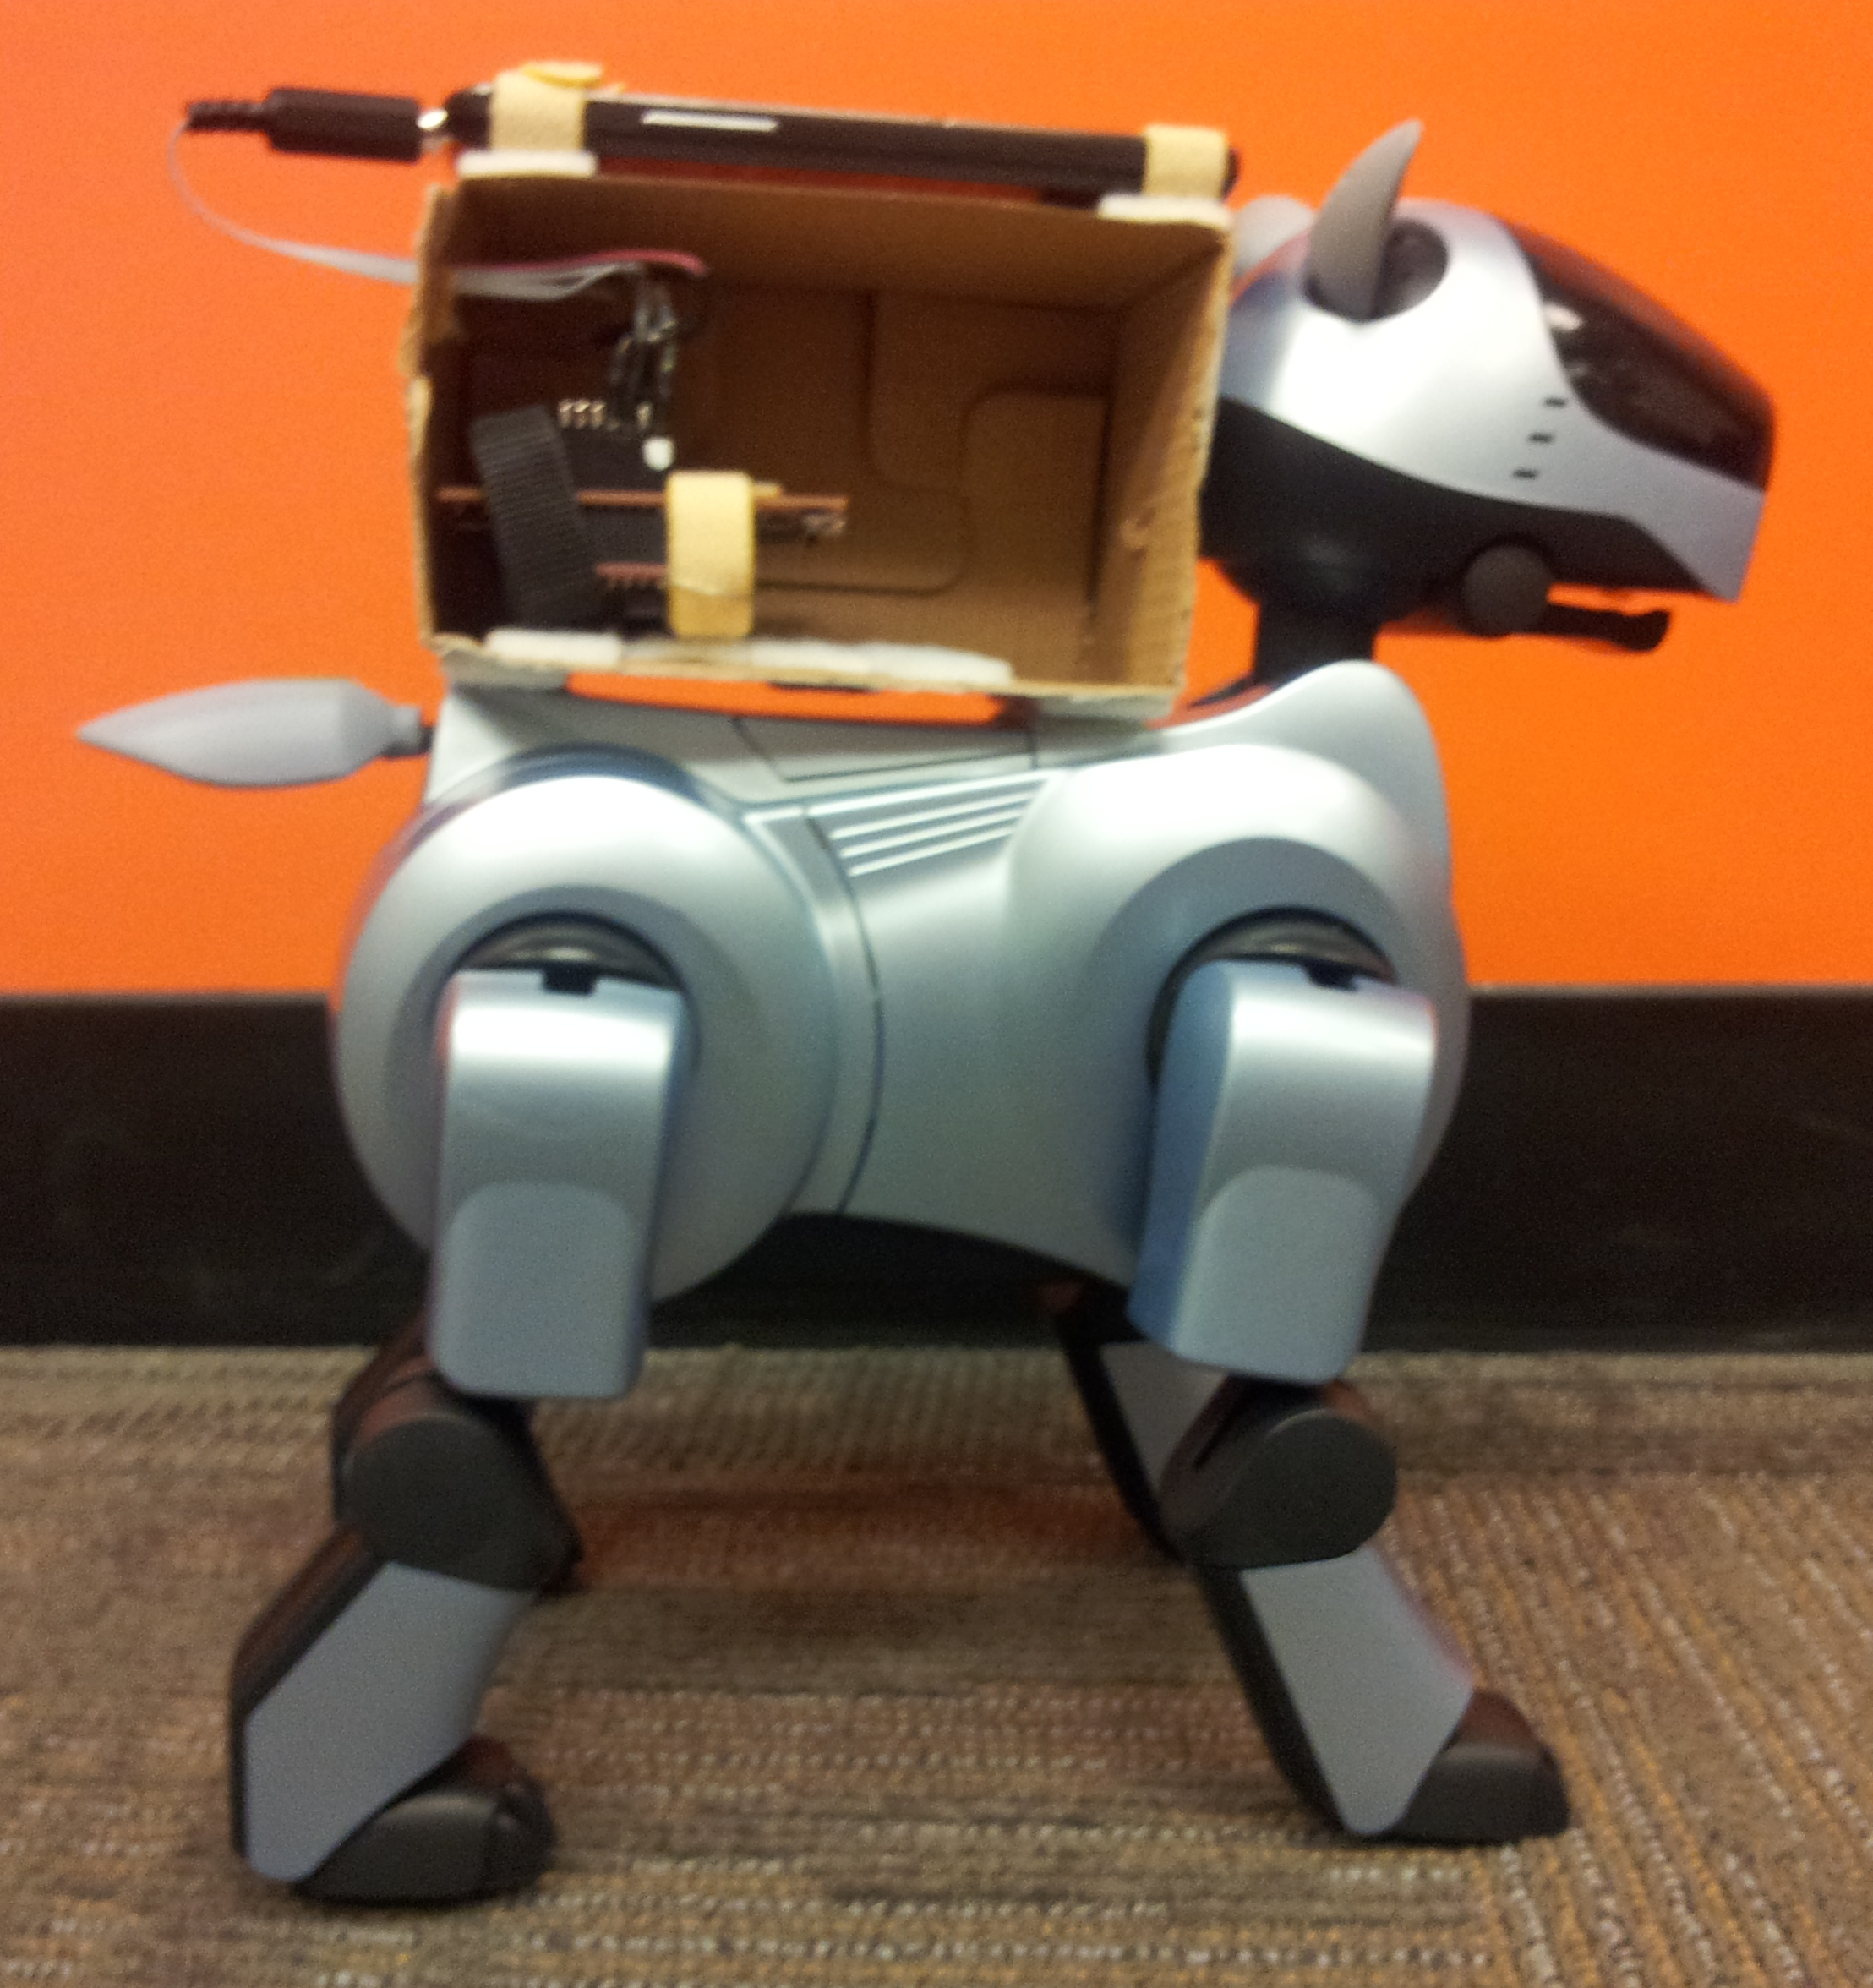
\includegraphics[width=3in]{aibo_ers_210.jpg}
	\caption{AIBO ERS 210 with Smartsensor prototype.}
	\label{fig:aibo}
\end{figure}

\subsection{Test Platform and Applications}
\label{sec:applications}

To enable us to conduct controlled and repeatable experiments, we
mounted the Smartsensor prototype on the back of an AIBO ERA 210 robot
dog (see Figure~\ref{fig:aibo}). Because the robot's actions can be
scripted, this setup provides an efficient and reliable way to
determine ground truth. In contrast, labelling data collected from
human subjects with ground truth is error prone and labour intensive.

We developed three applications that detect activities that the robot
can perform: walking, sitting and standing, headbutts. We chose these
actions because they have similar acceleration signatures to human
activities. A walking robot has a similar acceleration signature as
its human counterpart, though at a lower intensity. The headbutts are
meant to represent very infrequent human actions such as falling. We
found that robot stance transitions between the normal and sitting
postures are very similar in their acceleration signature to humans
sitting down and standing up. In Section~\ref{sec:results} we show
that the energy saving measured in our experiments with the robot
approximate closely the results of experiments conducted on limited
traces collected from human subjects.

\paragraph{Steps} Counts how many steps the robot takes when it
  walks. It's algorithm is based on the human step detection algorithm
  proposed by Ryan Libby in~\cite{libbyFootstepDetection}. The
  application takes in raw accelerometer readings and applies a
  low-pass filter on the x-axis acceleration. It then searches for
  local maxima in the filtered x-axis acceleration. Local maxima
  between $2.5\:m/s^2$ and $4.5\:m/s^2$ are detected as steps, given
  that no other steps were detected within the last 100 ms.

\paragraph{Transitions} Detects transitions between sitting and
  standing.  The application monitors changes in acceleration due to
  gravity on the y and z axes to determine the orientation of the
  device. If the z-axis (up-down relative to the dog) acceleration is
  between $9 m/s^2$ and $11 m/s^2$, and the acceleration on the y-axis
  (front-back relative to the dog) is between $-1 m/s^2$ and $1
  m/s^2$, the device is in a horizontal position and the robot is
  assumed to be in a standing posture. Similarly, if the z-axis
  acceleration is between $7.5 m/s^2$ and $9.5 m/s^2$, and the
  acceleration on the y-axis is between $3.5 m/s^2$ and $5.5 m/s^2$,
  the device is in an angled position and the robot is assumed to be
  in a sitting posture. The application detects transitions by looking
  for posture changes.

\paragraph{Headbutts} Detects a sudden forward head movement.  The
  application monitors the y-axis acceleration and searches for local
  minima between $-3.75\:m/s^2$ and $-6.75\:m/s^2$.
